\documentclass[10pt,landscape]{article}
\usepackage{graphicx}
\usepackage{amssymb,amsmath,amsthm,amsfonts}
\usepackage{multicol,multirow}
\usepackage{calc}
\usepackage{ifthen}
\usepackage[landscape]{geometry}
\usepackage[colorlinks=true,citecolor=blue,linkcolor=blue]{hyperref}


\ifthenelse{\lengthtest { \paperwidth = 11in}}
    { \geometry{top=.5in,left=.5in,right=.5in,bottom=.5in} }
	{\ifthenelse{ \lengthtest{ \paperwidth = 297mm}}
		{\geometry{top=1cm,left=1cm,right=1cm,bottom=1cm} }
		{\geometry{top=1cm,left=1cm,right=1cm,bottom=1cm} }
	}
\pagestyle{empty}
\makeatletter
\renewcommand{\section}{\@startsection{section}{1}{0mm}%
                                {-1ex plus -.5ex minus -.2ex}%
                                {0.5ex plus .2ex}%x
                                {\normalfont\large\bfseries}}
\renewcommand{\subsection}{\@startsection{subsection}{2}{0mm}%
                                {-1explus -.5ex minus -.2ex}%
                                {0.5ex plus .2ex}%
                                {\normalfont\normalsize\bfseries}}
\renewcommand{\subsubsection}{\@startsection{subsubsection}{3}{0mm}%
                                {-1ex plus -.5ex minus -.2ex}%
                                {1ex plus .2ex}%
                                {\normalfont\small\bfseries}}
\makeatother
\setcounter{secnumdepth}{0}
\setlength{\parindent}{0pt}
\setlength{\parskip}{0pt plus 0.5ex}
% -----------------------------------------------------------------------

\title{Chocolate Chip Cookies}

\begin{document}

\raggedright
\footnotesize

\begin{center}
     \Large{\textbf{Chocolate Chip Cookies}} \\
     \small{\today}
\end{center}
\begin{multicols}{3}


\section{Notes}
\begin{tabular}{l l} 
 Yields & 32 Cookies \\ 
 Prep Time & 20 minutes \\ 
 Chill Time & 24 hours \\ 
 Cook Time & 12 minutes \\
 Bake Temperature & 325\textdegree F \\
 Room Temperature & Cold day
\end{tabular}

\bigskip

\section{Ingredients}
\begin{tabular}{l l} 
 All Purpose Flour & 560g \\ 
 Baking Soda & 2 tsp \\ 
 Cornstarch & 3 tsp \\ 
 Salt & 1 tsp  \\ 
 Unsalted Butter & 340g \\
 Brown Sugar & 300g \\
 Whole Egg & 2 \\
 Egg Yolk & 2 \\
 Milk & 5 tbsp \\
 Vanilla Extract & 4 tsp \\
 Semi Sweet Chocolate Chips & 1 cup \\
 Walnuts & 2 handful \\
\end{tabular}

\vfill\null
\columnbreak

\section{Instructions}
\begin{enumerate}
    \item Whisk the flour, baking soda, cornstarch, and salt together in a large bowl. Set aside.
    \item Whisk the melted butter, brown sugar, and granulated sugar together until no brown sugar lumps remain. Whisk in the egg, then the egg yolk. Finally, whisk in the vanilla extract.
    \item Pour the wet ingredients into the dry ingredients and mix together
    \item Add some milk to the wet bowl to pour out all the wet ingredients
    \item Fold in the chocolate and walnut chunks
    \item Chill dough in refrigerator for 24 hours
    \item Put dough out and bring it to room temperature
    \item Make small dough balls and press them onto cookie sheet
    \item Bake for 12 minutes at 325\textdegree F
    \item Turn off oven and allow them to cool inside the oven
\end{enumerate}
\bigskip
CAUTION: Raw cookie dough might be delicious but dangerous
\vfill\null
\columnbreak
 
\section{Results}
\begin{itemize}
    \item Cookies that were left in the oven on the bottom rack for 17 minutes were burnt
    \item Cookies that were left in the oven on the top rack for 8 minutes were under-cooked and required additional cooking at the end
    \item Cookies that were left in the oven on the top rack for 17 minutes were fine
    \item Cooling cookies inside oven resulted in crunchy cookies
    \item Right amount of sweetness 
    \item Significantly lacked chocolate chips
    \item Increased in height but not in width due to less butter
\end{itemize}
\bigskip
\section{Try out next batch}
\begin{itemize}
    \item Add more chocolate chips
    \item Use top rack if possible
    \item Cool cookies outside rather than in oven
\end{itemize}
\vfill\null
\columnbreak
\end{multicols}

\section{Images}
\newcommand{\widthsize}{3.3cm}
\begin{multicols}{3}
\subsection{Bottom Rack Extended Time}
\begin{tabular}{c c}
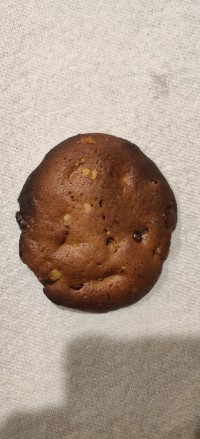
\includegraphics[width=\widthsize]{g1.jpg}&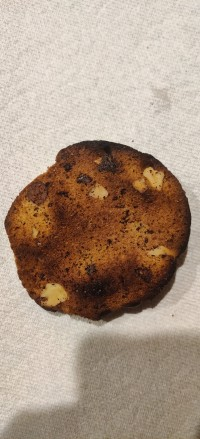
\includegraphics[width=\widthsize]{g2.jpg}\\
\end{tabular}

\subsection{Bottom Rack Decreased Time}
\begin{tabular}{c c}
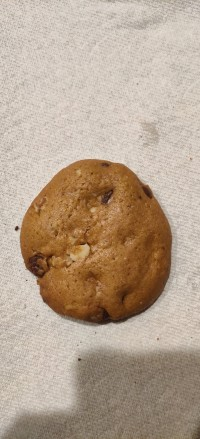
\includegraphics[width=\widthsize]{g3.jpg}&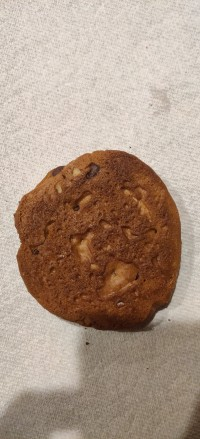
\includegraphics[width=\widthsize]{g4.jpg}\\
\end{tabular}

\subsection{Top Rack}
\begin{tabular}{c c}
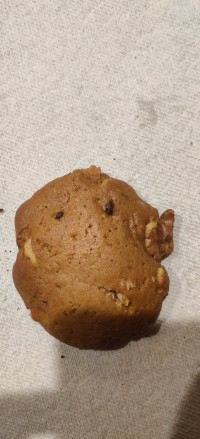
\includegraphics[width=\widthsize]{g5}&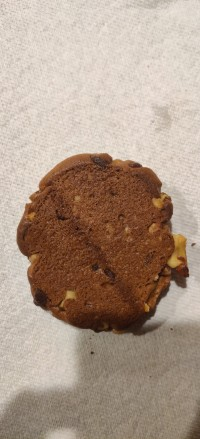
\includegraphics[width=\widthsize]{g6.jpg}\\
\end{tabular}

\end{multicols}

\bigskip
Inspired from \href{http://divisbyzero.com/}{https://sallysbakingaddiction.com/chewy-chocolate-chip-cookies/}
\end{document}
